\chapter{\textbf{Mathematical Modeling}}
As the system focuses on gas concentration-based alerting and control of appliances, thus only MQ-6 gas sensor calibration is considered for the mathematical analysis. DHT-11 sensor is to for checking the conditional Temperature and Relative Humidity.

\begin{figure}[h]
  \centering
  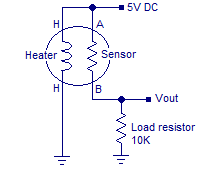
\includegraphics[width=2in]{14}
  \caption{MQ-6 Equivalent Circuit.}\label{fig14}
\end{figure}

\begin{justify}
Let, V\textsubscript{C} = Supply Voltage = +5V
\end{justify}\par

\begin{justify}
R\textsubscript{S} = Sensor Resistance
\end{justify}\par

\begin{justify}
R\textsubscript{L} = Load Resistance (Variable)
\end{justify}\par

\begin{justify}
V\textsubscript{out} = Sensor output Voltage
\end{justify}\par

\begin{justify}
From, Current flow and Voltage relationship,\ \ \ \ \ \ \ \ \ \ \ \ \ \ \ \ \ \ \ \ \ \ \ \ \ \ \ \ \ \ \ \ \ \
\end{justify}\par

\begin{equation}\label{5.1}
  V=I \times R
\end{equation}

\begin{equation*}
  ( V_{out}=\frac{Analog value \times 5}{1023})
\end{equation*}


Resistance of the sensor () is defined in datasheet [38] of MQ-6 as:\par

\begin{equation}\label{5.2}
  R_{s}= \left( \frac{V_{cc}}{V_{out}}-1 \right)  \times R_{L}= \left( \frac{1023}{Analog value}-1 \right)  \times R_{L}
\end{equation}

\vspace{\baselineskip}
Fresh air resistance ration for gas sensors: [38]\par

\begin{justify}
Data analyzing from R\textsubscript{S}/R\textsubscript{0} vs ppm graph: From the equations of a straight line,
\end{justify}\par



%%%%%%%%%%%%%%%%%%%% Table No: 1 starts here %%%%%%%%%%%%%%%%%%%%

\begin{equation}\label{5.3}
  y=mx+b
\end{equation}


%%%%%%%%%%%%%%%%%%%% Table No: 1 ends here %%%%%%%%%%%%%%%%%%%%

\begin{justify}
Here, y = value on Y-axis; x = value on X-axis; m = Slope of line; b = Intercept from Y-axis
\end{justify}\par

\begin{justify}
For log-log plot equation-(5) becomes:
\end{justify}\par


\begin{equation}\tag{5.4}
log \left( y \right) =m \times log \left( x \right) +b
\end{equation}
\begin{justify}
Note: the log is base 10.
\end{justify}\par

\begin{justify}
Slope (m) Value formula: If (x\textsubscript{0}, y\textsubscript{0}) and (x, y) are any two points of a line from a log-log plot then the formula for determining m is below:
\end{justify}\par


\begin{equation}\tag{5.5}
m=\frac{log_{10} \left( \frac{y}{y_{0}} \right) }{log_{10} \left( \frac{x}{x_{0}} \right) }
\end{equation}
\begin{justify}
Intercept from Y-axis (b) Value formula:
\end{justify}\par

\begin{justify}
From, equation-(5.6);
\end{justify}\par

\begin{equation*}
 ( log_{10} \left( y \right) =m \times log_{10} \left( x \right) +b)
\end{equation*}


\begin{equation}\tag{5.6}
Or, b=log_{10} \left( y \right) -m \times log_{10} \left( x \right)
\end{equation}
\begin{justify}
Using equations-(1) to (8) the gas concentration can be\textbf{ }determined directly in ppm (Parts per millions)
\end{justify}\par


\begin{equation}\tag{5.7}
log_{10} \left( ppm \right) =\frac{ \left( log_{10} \left( \frac{R_{s}}{R_{0}} \right) -b \right) }{m}
\end{equation}
From the MQ-6 datasheet we have obtained the value of m and b from equation (5.5) and (5.6)\par

\setlength{\parskip}{0.0pt}
Slope, m  \( = -0.423 \) \  \par

And b  \( =1.276 \)  \par

And sensor resistance  \( R_{0} \) =5.62  \( k \Omega  \) \par


\vspace{\baselineskip}
\setlength{\parskip}{8.04pt}
\par


\vspace{\baselineskip}
\setlength{\parskip}{0.0pt}


%%%%%%%%%%%%%%%%%%%% Table No: 2 starts here %%%%%%%%%%%%%%%%%%%%


\begin{table}[H]
\caption{Raw voltage values received through the MQ-6 sensor and corresponding temperature and humidity values:}
 			\centering
\begin{tabular}{p{0.23in}p{1.24in}p{1.55in}p{1.18in}p{1.37in}}
\hline
%row no:1
\multicolumn{1}{|p{0.23in}}{\Centering ID} &
\multicolumn{1}{|p{1.24in}}{\Centering Time} &
\multicolumn{1}{|p{1.55in}}{\Centering Temperature (in $ ^{\circ} $ C)} &
\multicolumn{1}{|p{1.18in}}{\Centering Humidity (in $\%$ )} &
\multicolumn{1}{|p{1.37in}|}{\Centering Analog value} \\
\hhline{-----}
%row no:2
\multicolumn{1}{|p{0.23in}}{\Centering 1} &
\multicolumn{1}{|p{1.24in}}{\Centering 13:19:41} &
\multicolumn{1}{|p{1.55in}}{\Centering 30} &
\multicolumn{1}{|p{1.18in}}{\Centering 61} &
\multicolumn{1}{|p{1.37in}|}{\Centering 533.15} \\
\hhline{-----}
%row no:3
\multicolumn{1}{|p{0.23in}}{\Centering 2} &
\multicolumn{1}{|p{1.24in}}{\Centering 13:19:36} &
\multicolumn{1}{|p{1.55in}}{\Centering 30} &
\multicolumn{1}{|p{1.18in}}{\Centering 61} &
\multicolumn{1}{|p{1.37in}|}{\Centering 533.48} \\
\hhline{-----}
%row no:4
\multicolumn{1}{|p{0.23in}}{\Centering 3} &
\multicolumn{1}{|p{1.24in}}{\Centering 13:19:31} &
\multicolumn{1}{|p{1.55in}}{\Centering 30} &
\multicolumn{1}{|p{1.18in}}{\Centering 61} &
\multicolumn{1}{|p{1.37in}|}{\Centering 532.48} \\
\hhline{-----}
%row no:5
\multicolumn{1}{|p{0.23in}}{\Centering 4} &
\multicolumn{1}{|p{1.24in}}{\Centering 13:19:25} &
\multicolumn{1}{|p{1.55in}}{\Centering 30} &
\multicolumn{1}{|p{1.18in}}{\Centering 61} &
\multicolumn{1}{|p{1.37in}|}{\Centering 528.04} \\
\hhline{-----}
%row no:6
\multicolumn{1}{|p{0.23in}}{\Centering 5} &
\multicolumn{1}{|p{1.24in}}{\Centering 13:19:20} &
\multicolumn{1}{|p{1.55in}}{\Centering 30} &
\multicolumn{1}{|p{1.18in}}{\Centering 61} &
\multicolumn{1}{|p{1.37in}|}{\Centering 532.48} \\
\hhline{-----}
%row no:7
\multicolumn{1}{|p{0.23in}}{\Centering 6} &
\multicolumn{1}{|p{1.24in}}{\Centering 13:19:15} &
\multicolumn{1}{|p{1.55in}}{\Centering 30} &
\multicolumn{1}{|p{1.18in}}{\Centering 61} &
\multicolumn{1}{|p{1.37in}|}{\Centering 532.48} \\
\hhline{-----}
%row no:8
\multicolumn{1}{|p{0.23in}}{\Centering 7} &
\multicolumn{1}{|p{1.24in}}{\Centering 13:19:10} &
\multicolumn{1}{|p{1.55in}}{\Centering 30} &
\multicolumn{1}{|p{1.18in}}{\Centering 61} &
\multicolumn{1}{|p{1.37in}|}{\Centering 528.04} \\
\hhline{-----}
%row no:9
\multicolumn{1}{|p{0.23in}}{\Centering 8} &
\multicolumn{1}{|p{1.24in}}{\Centering 13:19:05} &
\multicolumn{1}{|p{1.55in}}{\Centering 30} &
\multicolumn{1}{|p{1.18in}}{\Centering 61} &
\multicolumn{1}{|p{1.37in}|}{\Centering 528.04} \\
\hhline{-----}
%row no:10
\multicolumn{1}{|p{0.23in}}{\Centering 9} &
\multicolumn{1}{|p{1.24in}}{\Centering 13:18:59} &
\multicolumn{1}{|p{1.55in}}{\Centering 30} &
\multicolumn{1}{|p{1.18in}}{\Centering 61} &
\multicolumn{1}{|p{1.37in}|}{\Centering 528.04} \\
\hhline{-----}
%row no:11
\multicolumn{1}{|p{0.23in}}{\Centering 10} &
\multicolumn{1}{|p{1.24in}}{\Centering 13:18:54} &
\multicolumn{1}{|p{1.55in}}{\Centering 30} &
\multicolumn{1}{|p{1.18in}}{\Centering 61} &
\multicolumn{1}{|p{1.37in}|}{\Centering 528.04} \\
\hhline{-----}

\end{tabular}
 \end{table}


%%%%%%%%%%%%%%%%%%%% Table No: 2 ends here %%%%%%%%%%%%%%%%%%%%


\vspace{\baselineskip}
\setlength{\parskip}{8.04pt}
\par



%%%%%%%%%%%%%%%%%%%% Table No: 3 starts here %%%%%%%%%%%%%%%%%%%%


\begin{table}[H]
\caption{The Temperature and Humidity correction factor is used and the Corrected Resistance and subsequently the Corrected PPM is evaluated: [69]}
\label{tab:5. 3 The Temperature and Humidity correction factor is used and the Corrected Resistance and subsequently the Corrected PPM is evaluated: [69]}
 			\centering
\begin{tabular}{p{0.23in}p{1.24in}p{1.55in}p{2.74in}}
\hline
%row no:1
\multicolumn{1}{|p{0.23in}}{\Centering ID} &
\multicolumn{1}{|p{1.24in}}{\Centering Time} &
\multicolumn{1}{|p{1.55in}}{\Centering Resistance ( \( R_{s} \) )} &
\multicolumn{1}{|p{2.74in}|}{\Centering PPM} \\
\hhline{----}
%row no:2
\multicolumn{1}{|p{0.23in}}{\Centering 1} &
\multicolumn{1}{|p{1.24in}}{\Centering 13:19:41} &
\multicolumn{1}{|p{1.55in}}{\Centering 9187.764} &
\multicolumn{1}{|p{2.74in}|}{\Centering 325} \\
\hhline{----}
%row no:3
\multicolumn{1}{|p{0.23in}}{\Centering 2} &
\multicolumn{1}{|p{1.24in}}{\Centering 13:19:36} &
\multicolumn{1}{|p{1.55in}}{\Centering 9175.828} &
\multicolumn{1}{|p{2.74in}|}{\Centering 316} \\
\hhline{----}
%row no:4
\multicolumn{1}{|p{0.23in}}{\Centering 3} &
\multicolumn{1}{|p{1.24in}}{\Centering 13:19:31} &
\multicolumn{1}{|p{1.55in}}{\Centering 9211.781} &
\multicolumn{1}{|p{2.74in}|}{\Centering 313} \\
\hhline{----}
%row no:5
\multicolumn{1}{|p{0.23in}}{\Centering 4} &
\multicolumn{1}{|p{1.24in}}{\Centering 13:19:25} &
\multicolumn{1}{|p{1.55in}}{\Centering 9373.252} &
\multicolumn{1}{|p{2.74in}|}{\Centering 310} \\
\hhline{----}
%row no:6
\multicolumn{1}{|p{0.23in}}{\Centering 5} &
\multicolumn{1}{|p{1.24in}}{\Centering 13:19:20} &
\multicolumn{1}{|p{1.55in}}{\Centering 9211.781} &
\multicolumn{1}{|p{2.74in}|}{\Centering 313} \\
\hhline{----}
%row no:7
\multicolumn{1}{|p{0.23in}}{\Centering 6} &
\multicolumn{1}{|p{1.24in}}{\Centering 13:19:15} &
\multicolumn{1}{|p{1.55in}}{\Centering 9211.781} &
\multicolumn{1}{|p{2.74in}|}{\Centering 313} \\
\hhline{----}
%row no:8
\multicolumn{1}{|p{0.23in}}{\Centering 7} &
\multicolumn{1}{|p{1.24in}}{\Centering 13:19:10} &
\multicolumn{1}{|p{1.55in}}{\Centering 9373.252} &
\multicolumn{1}{|p{2.74in}|}{\Centering 310} \\
\hhline{----}
%row no:9
\multicolumn{1}{|p{0.23in}}{\Centering 8} &
\multicolumn{1}{|p{1.24in}}{\Centering 13:19:05} &
\multicolumn{1}{|p{1.55in}}{\Centering 9373.252} &
\multicolumn{1}{|p{2.74in}|}{\Centering 310} \\
\hhline{----}
%row no:10
\multicolumn{1}{|p{0.23in}}{\Centering 9} &
\multicolumn{1}{|p{1.24in}}{\Centering 13:18:59} &
\multicolumn{1}{|p{1.55in}}{\Centering 9373.252} &
\multicolumn{1}{|p{2.74in}|}{\Centering 310} \\
\hhline{----}
%row no:11
\multicolumn{1}{|p{0.23in}}{\Centering 10} &
\multicolumn{1}{|p{1.24in}}{\Centering 13:18:54} &
\multicolumn{1}{|p{1.55in}}{\Centering 9373.252} &
\multicolumn{1}{|p{2.74in}|}{\Centering 310} \\
\hhline{----}

\end{tabular}
 \end{table}


%%%%%%%%%%%%%%%%%%%% Table No: 3 ends here %%%%%%%%%%%%%%%%%%%%


\vspace{\baselineskip}
\par


\begin{equation}\tag{5.8}
R_{s} \_ Scaling factor=1.6979-0.012t-0.00612h
\end{equation}
\begin{equation*}
   (  Corrected R_{s}= \frac{R_{s}}{R_{s} \_ Scaling factor})
\end{equation*}




%%%%%%%%%%%%%%%%%%%% Table No: 4 starts here %%%%%%%%%%%%%%%%%%%%


\begin{table}[H]
\caption{The Temperature and Humidity correction factor is used and the Corrected Resistance and subsequently the Corrected PPM is evaluated: [69]}
 			\centering
\begin{tabular}{p{0.23in}p{1.24in}p{1.68in}p{1.05in}p{1.37in}}
\hline
%row no:1
\multicolumn{1}{|p{0.23in}}{\Centering ID} &
\multicolumn{1}{|p{1.24in}}{\Centering Time} &
\multicolumn{1}{|p{1.68in}}{\Centering Resistance Corrected  \( R_{s} \) } &
\multicolumn{1}{|p{1.05in}}{\Centering Corrected PPM} &
\multicolumn{1}{|p{1.37in}|}{\Centering Correction Factor} \\
\hhline{-----}
%row no:2
\multicolumn{1}{|p{0.23in}}{\Centering 1} &
\multicolumn{1}{|p{1.24in}}{\Centering 13:19:41} &
\multicolumn{1}{|p{1.68in}}{\Centering 7177.940} &
\multicolumn{1}{|p{1.05in}}{\Centering 582.55} &
\multicolumn{1}{|p{1.37in}|}{\Centering 1.28} \\
\hhline{-----}
%row no:3
\multicolumn{1}{|p{0.23in}}{\Centering 2} &
\multicolumn{1}{|p{1.24in}}{\Centering 13:19:36} &
\multicolumn{1}{|p{1.68in}}{\Centering 7168.615} &
\multicolumn{1}{|p{1.05in}}{\Centering 584.34} &
\multicolumn{1}{|p{1.37in}|}{\Centering 1.28} \\
\hhline{-----}
%row no:4
\multicolumn{1}{|p{0.23in}}{\Centering 3} &
\multicolumn{1}{|p{1.24in}}{\Centering 13:19:31} &
\multicolumn{1}{|p{1.68in}}{\Centering 7196.703} &
\multicolumn{1}{|p{1.05in}}{\Centering 578.96} &
\multicolumn{1}{|p{1.37in}|}{\Centering 1.28} \\
\hhline{-----}
%row no:5
\multicolumn{1}{|p{0.23in}}{\Centering 4} &
\multicolumn{1}{|p{1.24in}}{\Centering 13:19:25} &
\multicolumn{1}{|p{1.68in}}{\Centering 7338.478} &
\multicolumn{1}{|p{1.05in}}{\Centering 552.87} &
\multicolumn{1}{|p{1.37in}|}{\Centering 1.28} \\
\hhline{-----}
%row no:6
\multicolumn{1}{|p{0.23in}}{\Centering 5} &
\multicolumn{1}{|p{1.24in}}{\Centering 13:19:20} &
\multicolumn{1}{|p{1.68in}}{\Centering 7196.703} &
\multicolumn{1}{|p{1.05in}}{\Centering 578.96} &
\multicolumn{1}{|p{1.37in}|}{\Centering 1.28} \\
\hhline{-----}
%row no:7
\multicolumn{1}{|p{0.23in}}{\Centering 6} &
\multicolumn{1}{|p{1.24in}}{\Centering 13:19:15} &
\multicolumn{1}{|p{1.68in}}{\Centering 7196.703} &
\multicolumn{1}{|p{1.05in}}{\Centering 578.96} &
\multicolumn{1}{|p{1.37in}|}{\Centering 1.28} \\
\hhline{-----}
%row no:8
\multicolumn{1}{|p{0.23in}}{\Centering 7} &
\multicolumn{1}{|p{1.24in}}{\Centering 13:19:10} &
\multicolumn{1}{|p{1.68in}}{\Centering 7338.478} &
\multicolumn{1}{|p{1.05in}}{\Centering 552.87} &
\multicolumn{1}{|p{1.37in}|}{\Centering 1.28} \\
\hhline{-----}
%row no:9
\multicolumn{1}{|p{0.23in}}{\Centering 8} &
\multicolumn{1}{|p{1.24in}}{\Centering 13:19:05} &
\multicolumn{1}{|p{1.68in}}{\Centering 7338.478} &
\multicolumn{1}{|p{1.05in}}{\Centering 552.87} &
\multicolumn{1}{|p{1.37in}|}{\Centering 1.28} \\
\hhline{-----}
%row no:10
\multicolumn{1}{|p{0.23in}}{\Centering 9} &
\multicolumn{1}{|p{1.24in}}{\Centering 13:18:59} &
\multicolumn{1}{|p{1.68in}}{\Centering 7338.478} &
\multicolumn{1}{|p{1.05in}}{\Centering 552.87} &
\multicolumn{1}{|p{1.37in}|}{\Centering 1.28} \\
\hhline{-----}
%row no:11
\multicolumn{1}{|p{0.23in}}{\Centering 10} &
\multicolumn{1}{|p{1.24in}}{\Centering 13:18:54} &
\multicolumn{1}{|p{1.68in}}{\Centering 7338.478} &
\multicolumn{1}{|p{1.05in}}{\Centering 552.87} &
\multicolumn{1}{|p{1.37in}|}{\Centering 1.28} \\
\hhline{-----}

\end{tabular}
 \end{table}


%%%%%%%%%%%%%%%%%%%% Table No: 4 ends here %%%%%%%%%%%%%%%%%%%%



\section{Algorithm of the process }
\setlength{\parskip}{0.0pt}
\textcolor[HTML]{111111}{setup( )}\par

\textcolor[HTML]{111111}{$ \{ $  setAnalogPinforMQ135(analog0);}\par

\textcolor[HTML]{111111}{setAnalogP}\par

\textcolor[HTML]{111111}{inforDHT11(analog1);}\par

\textcolor[HTML]{111111}{Serial.begin(9600);}\par

\textcolor[HTML]{111111}{$ \} $ }\par

\textcolor[HTML]{111111}{loop( )}\par

\textcolor[HTML]{111111}{$ \{ $ \  AnalogValue = receiveMQdata( );}\par

T = TempfromDHT11( );\par

H = HumfromDHT11( );\par

Vout= convertanalogtovoltage(AnalogValue);\par

while(calibrationisnotcomplete)\par

$ \{ $  RO= calculateRoValue(Vout, DefaultPPM);$ \} $ \par

RS= calculateRsValue(CaliberatedRO, Vout);\par

CorrectedRS= TempHumCalibRs(RS, T, H);\par

ppm = PPM(RS, RO, MQ\_Scaling\_Factor, MQ\_Exponent\_Factor); \par

Correctedppm = PPM(CorrectedRS, RO, MQ\_Scaling\_Factor, MQ\_Exponent\_Factor);\par

PlotDatainMatlab( );\par

SendDatatoSerialMonitor( );\par

SendDatatoExcel( );\par

$ \} $ \par

\setlength{\parskip}{8.04pt}
\section{Calculation of the solar PV energy output of a photovoltaic cell [70]}
\begin{justify}
We construct a solar panel which is used for powering the controller. A dimension about 11.5cm \(   \times  \)  6 cm rectangular solar plate is used to make the solar panel.
\end{justify}\par



%%%%%%%%%%%%%%%%%%%% Table No: 5 starts here %%%%%%%%%%%%%%%%%%%%

%
%\begin{table}[H]
% 			\centering
%\begin{tabular}{p{1.69in}p{1.6in}p{2.8in}}
%%row no:1
%\multicolumn{1}{p{1.69in}}{\textbf{Global formula:}} &
%\multicolumn{1}{p{1.6in}}{ \( E=A \times r \times H \times PR \) \ \  } &
%\multicolumn{1}{p{2.8in}}{(5.9)} \\
%\hhline{~~~}
%
%\end{tabular}
% \end{table}
 \begin{equation}\tag{5.9}
\textbf{Global formula}:Energy,E=A \times r \times H \times PR
\end{equation}


%%%%%%%%%%%%%%%%%%%% Table No: 5 ends here %%%%%%%%%%%%%%%%%%%%


\vspace{\baselineskip}


%%%%%%%%%%%%%%%%%%%% Table No: 6 starts here %%%%%%%%%%%%%%%%%%%%


\begin{table}[H]
 			\centering
\begin{tabular}{p{5.13in}p{1.15in}}
\hline
%row no:1
\multicolumn{1}{|p{5.13in}}{E = Energy (kWh)\ \  \ \ \ \ \ \ \ \ \  } &
\multicolumn{1}{|p{1.15in}|}{ kWh/an} \\
\hhline{--}
%row no:2
\multicolumn{1}{|p{5.13in}}{A = Total solar panel Area $(m^2)$} &
\multicolumn{1}{|p{1.15in}|}{0.0069 $m^2$} \\
\hhline{--}
%row no:3
\multicolumn{1}{|p{5.13in}}{r = solar panel yield ($\%$ )} &
\multicolumn{1}{|p{1.15in}|}{15$\%$ } \\
\hhline{--}
%row no:4
\multicolumn{1}{|p{5.13in}}{H = Annual average irradiation on tilted panel (shadings not included) $\ast$ } &
\multicolumn{1}{|p{1.15in}|}{ $kWh/m^2.an$} \\
\hhline{--}
%row no:5
\multicolumn{1}{|p{5.13in}}{PR = Performance ratio, coefficient for losses (range between 0.9 and 0.5, default value =0.75)} &
\multicolumn{1}{|p{1.15in}|}{0.75} \\
\hhline{--}

\end{tabular}
 \end{table}


%%%%%%%%%%%%%%%%%%%% Table No: 6 ends here %%%%%%%%%%%%%%%%%%%%


\vspace{\baselineskip}
\section{Relative Humidity Calculation using DHT11 Sensor}

After getting start pulse from the controller, DHT11 sends the response pulse to the microcontroller which will indicate that DHT11 received start pulse.The response pulse is low for 54 microsecond and then goes high for 80 microsecond.
After sending the response pulse, DHT11 sensor sends the data, which contains humidity and temperature value along with checksum. The data frame is of total 40 bits long, it contains 5 segments (byte) and each segment is 8-bit long.In this 5 segments first two segments content humidity value in decimal integer form. This Value gives  Relative Percentage Humidity. 1st 8-bits are integer part and next 8 bits are fractional partNext two segment content temperature value in decimal integer form. This value gives us temperature in Celsius form.
Here checksum byte is direct addition of humidity and temperature value. And it would be verified using it in microcontroller whether it is same as checksum value or not. If it is not equal, then there is some error in the data value otherwise the data is correct.Once microcontroller receives data, DHT11 pin goes in low power consumption mode until the microcontroller do not sends start pulse again \cite{collotta2018bluetooth}.

\textbf{End-Pulse}:After sending 40-bit data, DHT11 sensor sends 54us low level and then goes high. After this DHT11 goes in sleep mode.
If the temperature and the dewpoint was knew, and wanted to obtain relative humidity, the formulas are as follows:\par
First, to convert the temperature and the dewpoint from Fahrenheit to Celsius, use the following formulas.\par

\begin{equation}\tag{5.10}
 T_{c}=\frac{5 \times  \left( T_{f}-32.0 \right) }{9}
\end{equation}

\begin{equation}\tag{5.11}
T_{dc}=\frac{5 \times  \left( T_{df}-32.0 \right) }{9}
\end{equation}
 \( T_{c} \) =air temperature in degrees Celsius,  \( T_{f} \) =air temperature in degrees Fahrenheit\par

 \( T_{dc} \) =dewpoint temperature in degrees Celsius\par

 \( T_{df} \) =dewpoint temperature in degrees Fahrenheit\par

The next set of formulas assumes a standard atmospheric pressure. These formulas will calculate saturation vapor pressure (Es) and actual vapor pressure(E) in millibars.\par


\begin{equation}\tag{5.12}
E_{s}=6.11 \times 10.0  \times  \left( \frac{7.5 \times T_{c}}{237.7+T_{c}} \right)
\end{equation}

\vspace{\baselineskip}
\setlength{\parskip}{0.0pt}

\begin{equation}\tag{5.13}
E=6.11 \times 10.0  \times  \left( \frac{7.5 \times T_{dc}}{237.7+T_{dc}} \right) \ \ \
\end{equation}
Once the saturation vapor pressure and the actual vapor pressure, relative humidity can be computed by dividing the actual vapor pressure by the saturation vapor pressure and then multiplying by 100 to convert the quantity to a percent.\par


\begin{equation}\tag{5.14}
Relative Humidity (RH) in percent =\frac{E}{E_{s}} \times 100\%
\end{equation}
For example, a station report that included an air temperature of 85 degrees Fahrenheit and a dewpoint of 65 degrees Fahrenheit and you wanted to compute the relative humidity, you would proceed as follows \cite{schafer2013accurate}.\\

First, convert the Fahrenheit values to Celsius using formulas. The values should be  \( T_{c} \) =29.4 and  \( T_{dc} \) =18.3\par

Next, calculate the saturation vapor pressure and the actual vapor pressure using formulas (5.12) and (5.13) respectively. The values should be  \( E_{s} \)  =40.9 and  \( E \)  =21.0\par

Finally, calculate relative humidity using formula (5.14). The final answer should be RH=51.3 $\%$ .\par
\section{Chapter Summery}
In this Chapter mathematical modelling of the sensor was derived and by using this calculation the analog voltage of the Gas sensor is converted into the PPM value as well as the temperature and the humidity also calculated using above described equations.This chapter also contains the solar equivalent energy which is provided to the controller for supplying power.  